\documentclass[a4paper,11pt]{article} %Sets the default text size to 11pt and class to article.
%------------------------Dimensions--------------------------------------------
\topmargin=0.0in %length of margin at the top of the page (1 inch added by default)
\oddsidemargin=0.0in %length of margin on sides for odd pages
\evensidemargin=0in %length of margin on sides for even pages
\textwidth=6.5in %How wide you want your text to be
\marginparwidth=0.5in
%\headheight=0pt %1in margins at top and bottom (1 inch is added to this value by default)
%\headsep=0pt %Increase to increase white space in between headers and the top of the page
\textheight=9.0in

\usepackage{graphicx}

\graphicspath{ {./} }
\begin{document}
\raggedleft
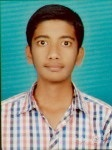
\includegraphics{photo}
\smallskip
\hrule
\smallskip
\raggedright
\textbf{{\Huge \sc Sanket Sunil Patil \newline}}
\smallskip
\textbf{\small Second Year, Computer Engineering, College of Engineering Pune, Pune.}
\bigskip

\hrule
\smallskip
\begin{minipage}[b]{0.9\textwidth}
			\raggedleft
			(+91)9860575626\par
			sanketsunilpatilsp@gmail.com\par
		\end{minipage}%

\begin{minipage}[b]{0.33333\textwidth}
			\raggedright
			"Suparshwa",Arihant Colony\par
			100 Ft Road, Sangli-416416\par
			Maharashtra, India
		\end{minipage}

\bigskip


\hrule
\bigskip
\raggedright
		\begin{LARGE}
				
				\textbf{\large $\ast$ Objective:}\medskip\linebreak%
				{\small An internship opportunity that will allow me to utilize my problem solving skills and learn new things to further develop my abilities in the field of computer science.\newline}\bigskip
		\end{LARGE}
\hrule	
\bigskip
\textbf{\large $\ast$ Education:}\smallskip\linebreak
\begin{center}
 \begin{tabular}{||c || c || c || c||} 
 \hline
 Course & Institution & Year of Passing & Score \\ [0.8ex] 
 \hline\hline
 S.Y. B-tech & College Of Engineering Pune, Pune. & 2018 - 2019 & Sem I : 8.71 \\ 
 \hline
 F.Y. B-tech & College Of Engineering Pune, Pune. & 2017 - 2018 & CPI     : 8.74 \\
 \hline
 HSC & G. A. College, Sangli. & 2016 - 2017 & 94.31 \%  (PCM 97.33 \%)\linebreak \\

 \hline
 SSC& City High School, Sangli. & 2014 - 2015 & 98.40 \% \\
 \hline

 \hline
\end{tabular}
\end{center}

			\begin{LARGE}
				\textbf{\large $\ast$ Projects:}\medskip%
				{\small
					\begin{enumerate}
						\item \textbf{Text Editor:} Terminal based Text Editor to create, edit \& save documents\newline
						Data Structures \& Algorithms
						\item \textbf{Online Hostel allotment system:} Hostel Allotement System as per merit \& Branch \newline
						 HTML | CSS | JS | MySQL
						\item \textbf{Hydroquadrotar Robot:} To inspect under water using robot and to automate task. \newline
						Embedded C
						\item \textbf{Face Unlock For Laptop:} Ongoing project. To recognize face of user to unlock the laptop.\newline
						Python | OpenCV| Machine Learning
						
						\item Maze solver using line follower , Image processing using Matlab for \textbf{Robocon'19}
					\end{enumerate}
					\bigskip
				}
			\end{LARGE}
\hrule	
\bigskip

			\begin{LARGE}
				\textbf{\large $\ast$ Training:}\medskip%
				{\small
					\begin{itemize}
						\item \textbf{INSPIRE}(Innovations in Science Pursuit for Inspired Research) : \newline
5 Days workshop organised at Willingdon College , Sangli.
					\end{itemize}
					\bigskip
				}
				
			\end{LARGE}			
\hrule	
\bigskip
			\begin{LARGE}
				\textbf{\large $\ast$ Technical skills:}\medskip%
				{\small
					\begin{itemize}
						\item C++, C, Python , Embedded C (Novice)
						\item  HTML, CSS, JavaScript(Novice), AngularJS(Novice)
						\item Web Development, Image Processing
						\item Algorithms \& Data structures, Competitive programming
					\end{itemize}
					\bigskip
				}
				
			\end{LARGE}
			\medskip
\hrule	
\bigskip

			\begin{LARGE}
				\textbf{\large $\ast$ Co-Curricular Activities:}\smallskip%
				{\small
					\begin{enumerate}%[leftmargin=*]
						\item \textbf{2nd Rank } at \textbf{E-Yantra Robotics Competition} 2k18 held at IIT - Bombay.
						\item \textbf{Runner up} in \textbf{Dogfight} event at Mindspark 2k18.
						\item Club Member of \textbf{Robotics Team of COEP} [Robot Study Circle].
						\item \textbf{Winner} of Annual Science Quiz 2k17
						\item \textbf{Finalist} in Mindspark Hackathon 2k18
						
						\item \textbf{State Rank 13} in MHTCET (2017), 1st in Sangli District
						\item \textbf{1st in Sangli District} in HSC, JEE(Main), JEE(Advanced)(March'17)\newline
						 JEE(MAIN) Score : 186 (AIR 11787) ,JEE(ADVANCED) Score : 160 (AIR 15115)
						
					\end{enumerate}
				}
			\end{LARGE}
\hrule	
\bigskip

\end{document}
